\documentclass{article}
\UseRawInputEncoding 
\usepackage[utf8]{inputenc} 
\usepackage[T1]{fontenc}   
\usepackage[polish]{babel}
\usepackage{listings} 
\usepackage{xcolor}  
\usepackage{graphicx} 
\usepackage{float}
\usepackage{hyperref}
\usepackage[a4paper, left=2.5cm, right=2.5cm]{geometry}

\lstset{
    basicstyle=\ttfamily\small,
    backgroundcolor=\color{gray!10},
    frame=single,
    breaklines=true,
    numbers=left,
    numberstyle=\tiny\color{gray},
    captionpos=b,
    language=bash
}


\title{Opis Projektu "Labirynt" \\ }
\author{(link do repozytorium github: \\ \url{https://github.com/AleksandraGrabowska04/labirynt.git})}

\begin{document}

\maketitle

\section{Cel projektu}
Celem projektu "Labirynt" jest sprawdzenie, jak różne algorytmy radzą sobie z rozwiązywaniem labiryntów. Projekt umożliwia użytkownikowi nie tylko generowanie i wizualizację labiryntów, ale także przeprowadzenie testów porównujących algorytmy takie jak DFS, BFS, Dijkstra i A*. Wyniki analiz są przedstawiane w formie wykresów, co pozwala lepiej zrozumieć różnice w ich działaniu pod względem wydajności oraz liczby wykonanych kroków potrzebnych do rozwiązania labiryntu.

\section{Opis projektu}
Projekt "Labirynt" to aplikacja, która pozwala na tworzenie, rozwiązywanie i analizowanie labiryntów za pomocą różnych algorytmów. Dzięki niej można generować labirynty o rozmiarach \(n \times n\) (gdzie \(n\) to liczba pól ściany labiryntu), rozwiązywać je automatycznie, a następnie wizualizować działanie algorytmów krok po kroku. Wyniki działania algorytmów są porównywane i prezentowane w formie wykresów, co ułatwia ich zrozumienie i ocenę.

\subsection{Funkcjonalności projektu}
\begin{enumerate}
    \item \textbf{Generowanie labiryntów}
    \begin{itemize}
        \item Możliwość tworzenia labiryntów o różnych wymiarach \(n \times n\).
        \item Labirynty są generowane w postaci macierzy (pól) zer i jedynek, a następnie przekształcane na grafy, w których pola to węzły, a ścieżki to połączenia między nimi.
        \item Labirynt zawsze ma jedno wejście (w lewym górnym rogu) i jedno wyjście (w prawym dolnym rogu).
    \end{itemize}
    
    \item \textbf{Rozwiązywanie labiryntów za pomocą algorytmów przeszukiwania}
    \begin{itemize}
        \item Zaimplementowano cztery algorytmy:
        \begin{itemize}
            \item \textbf{DFS (Depth-First Search)} – algorytm eksploruje jak najdalsze ścieżki, cofając się tylko w razie potrzeby. Jest szybki, ale nie zawsze znajduje najkrótszą ścieżkę.
            \item \textbf{BFS (Breadth-First Search)} – algorytm bada wszystkie możliwe ścieżki równolegle, co gwarantuje znalezienie najkrótszej drogi, ale jest bardziej czasochłonny.
            \item \textbf{Dijkstra} – algorytm przeszukujący grafy w sposób optymalny, uwzględniając koszt przejścia między węzłami (przydatny w przypadku labiryntów z różnymi wagami krawędzi).
            \item \textbf{A*} – algorytm heurystyczny, który stara się ''przewidzieć'', którędy idzie ścieżka do wyjścia na podstawie dostępnych dla niego danych.
        \end{itemize}
        \item Użytkownik może zobaczyć, jak każdy algorytm przeszukuje labirynt i jaką ścieżkę wybiera.
    \end{itemize}
    
    \item \textbf{Graficzna wizualizacja}
    \begin{itemize}
        \item Labirynty są rysowane w formie macierzy 2D, gdzie:
        \begin{itemize}
            \item 1 oznacza ścianę, gdzie cały labirynt jest otoczony ścianami,
            \item 0 oznacza wolne pole (ścieżka).
        \end{itemize}
        \item Proces przeszukiwania labiryntu można śledzić krok po kroku, co pozwala zobaczyć, jak algorytm podejmuje decyzje.
    \end{itemize}
    
    \item \textbf{Porównanie algorytmów}
    \begin{itemize}
        \item Po rozwiązaniu labiryntu projekt generuje pliki, które zawierają informacje takie jak:
        \begin{itemize}
            \item Liczba kroków wykonanych przez każdy algorytm.
            \item Odwiedzone węzły.
            \item Ścieżka rozwiązania labiryntu.
        \end{itemize}
        \item Następnie wyniki są prezentowane na wykresach (np. słupkowych lub liniowych), co ułatwia porównanie.
    \end{itemize}
\end{enumerate}

\subsection{Technologie użyte w projekcie}
\begin{itemize}
    \item \textbf{C/C++}
    \begin{itemize}
        \item Wykorzystywane do podstawowej logiki projektu, takiej jak:
        \begin{itemize}
            \item Generowanie labiryntów w postaci macierzy \(n \times n\).
            \item Implementacja algorytmów przeszukiwania.
            \item Zamiana macierzy labiryntu na postać grafu za pomocą struktury danych.
        \end{itemize}
    \end{itemize}
    
    \item \textbf{Python}
    \begin{itemize}
        \item Używany do:
        \begin{itemize}
            \item Generowania wykresów porównujących wyniki algorytmów za pomocą biblioteki Matplotlib.
            \item Obsługi analizy danych i ich wizualizacji.
        \end{itemize}
    \end{itemize}
    
    \item \textbf{Java}
    \begin{itemize}
        \item Stosowana do:
        \begin{itemize}
            \item Rysowania labiryntów z graficznym interfejsem użytkownika za pomocą Java2D.
            \item Wizualizacji kroków przeszukiwania w czasie rzeczywistym.
        \end{itemize}
    \end{itemize}
    
    \item \textbf{Lua i XMake}
    \begin{itemize}
        \item \textbf{Lua}: Język skryptowy używany do definiowania konfiguracji w pliku \texttt{xmake.lua}.
        \item \textbf{XMake}: Narzędzie do automatyzacji budowania projektu. W projekcie służy do:
        \begin{itemize}
            \item Konfigurowania i zarządzania procesem kompilacji aplikacji.
            \item Obsługi zależności projektu.
            \item Ułatwienia tworzenia wieloplatformowego kodu źródłowego (np. na Windows, Linux).
        \end{itemize}
        Skrypty w Lua umożliwiają prostą i czytelną definicję procesu budowania, co przyspiesza zarządzanie kompilacją w porównaniu z bardziej złożonymi narzędziami, takimi jak CMake.
    \end{itemize}
\end{itemize}

\section{Członkowie zespołu}
W skład zespołu pracującego nad projektem wchodzą:

\begin{itemize}
    \item Jakub Malinowski (lider zespołu)
    \begin{itemize}
        \item Nr indeksu: 288561
        \item Nazwa użytkownika na platformie GitHub: \texttt{at-eee}
    \end{itemize}
    \item Aleksandra Grabowska 
    \begin{itemize}
        \item Nr indeksu: 288559
        \item Nazwa użytkownika na platformie GitHub: \texttt{AleksandraGrabowska04}
    \end{itemize}
    \item Jakub Markowski
    \begin{itemize}
        \item Nr indeksu: 285709
        \item Nazwa użytkownika na platformie GitHub: \texttt{kuba913}
    \end{itemize}
    \item Krystian Dzikiewicz
    \begin{itemize}
        \item Nr indeksu: 289935
        \item Nazwa użytkownika na platformie GitHub: \texttt{LionDoge}
    \end{itemize}
\end{itemize}

\section{Podział pracy}

(Pełen podział pracy zmieniający się na przestrzeni czasu można zobaczyć wewnątrz pliku „\textit{podzial\_prac.md}” na stronie repozytorium projektu.)

\begin{itemize}
    \item Jakub Malinowski (at-eee):
    \begin{itemize}
        \item Koordynowanie projektem,
        \item Generowanie losowych labiryntów (w postaci macierzy),
        \item Zaprogramowanie algorytmu A* (A Gwiazdka) do rozwiązywania labiryntów.
    \end{itemize}
    \item Aleksandra Grabowska (AleksandraGrabowska04):
    \begin{itemize}
        \item Zaprogramowanie algorytmu Dijkstry do rozwiązywania labiryntów,
        \item Generowanie wykresów porównujących skuteczność wybranych algorytmów.
    \end{itemize}
    \item Jakub Markowski (kuba913):
    \begin{itemize}
        \item Graficzna reprezentacja labiryntu oraz demonstracja kroków wykonywanych przez algorytmy podczas obierania przez nich prawidłowych ścieżek szukających wyjścia z labiryntu.
    \end{itemize}
    \item Krystian Dzikiewicz (LionDoge):
    \begin{itemize}
        \item Opracowanie struktury danych przechowującej labirynt w postaci grafu,
        \item Zaprogramowanie algorytmu BFS i DFS do rozwiązywania labiryntów,
        \item Przygotowanie testów jednostkowych.
    \end{itemize}
\end{itemize}

\section{Instrukcja użytkowania}

\subsection{Wymagania wstępne}

Program działa zarówno na systemie \textit{Microsoft Windows} jak i \textit{Linux}, jednak do użytkowania zalecane jest korzystanie z systemu \textit{Linux} w dystrybucji \textit{Debian} (np. \textit{Ubuntu}). \\

Do uruchomienia programu jest wymagane następujące oprogramowanie/narzędzia:
\begin{itemize}
    \item xmake
    \item gcc i g++
    \item java
    \item python3
    \item matplotlib do python’a
\end{itemize}

Do ich zainstalowania na systemie Linux w dystrybucji debian (zalecane, ponieważ na nim głównie były wykonywane prace) możemy użyć w terminalu polecenia:

\begin{lstlisting}
sudo apt-get install xmake gcc g++ java python3
\end{lstlisting}

A następnie polecenia:

\begin{lstlisting}
pip install matplotlib
\end{lstlisting}

\subsection{Uruchomienie programu}

Następnie aby sklonować repozytorium (z: \url{https://github.com/AleksandraGrabowska04/labirynt.git}) wpisujemy w terminalu następujące polecenie:

\begin{lstlisting}
git clone https://github.com/AleksandraGrabowska04/labirynt.git
\end{lstlisting}

Potem aby uruchomić program:

\begin{lstlisting}
cd labirynt
xmake build
\end{lstlisting}

A następnie:

\begin{lstlisting}
xmake run labirynth [rozmiar(y) labiryntu/ow] [(opcjonalnie) nazwa docelowego folderu dla wynikow]
\end{lstlisting}

Na przykład:

\begin{lstlisting}
xmake run labirynth 30 60 120 240
\end{lstlisting}

\subsection{Uruchomienie reprezentacji graficznej (opcjonalne)}

Aby uruchomić graficzną reprezentację labiryntu i ścieżek rozwiązywanych przez algorytmy (musimy znajdować się w nadkatalogu katalogu projektowego (\textit{labirynt})):

\begin{lstlisting}
java -cp `./labirynt/target/classes' main/Main
\end{lstlisting}

\subsubsection{Obsługa okna programu do reprezentacji graficznej}

\begin{itemize}
        \item \textit{strzałka w prawo} - Przechodzi do graficznej reprezentacji następnego algorytmu.
        \item \textit{strzałka w lewo} - Wraca do graficznej reprezentacji poprzedniego algorytmu.
        \item \textit{spacja}: 
        \begin{itemize}
        	\item \textit{wciśnięta jednokrotnie} - odtworzenie przebiegu ściezki obieranej przez algorytm rozwiązujący labirynt.
        	\item \textit{wciśnięta jednokrotnie} - Przewinięcie do końca odtwarzania.
        	\item \textit{wciśnięta trzykrotnie} - powrót do stanu początkowego.
        \end{itemize}
\end{itemize}

\subsection{Utworzenie i uruchomienie wykresów porównujących (opcjonalne)}

Aby opcjonalnie uruchomić wykresy porównujące skuteczności algorytmów (musimy znajdować się w podkatalogu \textit{src}):

\begin{lstlisting}
python3 generate_plots.py
\end{lstlisting}

\subsubsection{Obsługa okien wykresów porównujących}

Obsługa okien jest intuicyjna i odbywa się za pomocą panelu użytkownika narzędzia \textit{matplotlib} znajdującego się w każdym z okienek (instrukcja obsługiwania nawigacji okien w matplotlib: \\ \url{https://matplotlib.org/3.2.2/users/navigation_toolbar.html}).

\section{Przykładowe uruchomienie z wykresami}

Przykładowa komenda:
\begin{lstlisting}[caption=Uruchamianie programu z różnymi rozmiarami labiryntów]
xmake run labyrinth 30 60 120 240
\end{lstlisting}

Uruchamia program, który generuje labirynty o wymiarach podanych w komendzie:
\begin{itemize}
    \item Labirynt o wymiarach $30 \times 30$,
    \item Labirynt o wymiarach $60 \times 60$,
    \item Labirynt o wymiarach $120 \times 120$,
    \item Labirynt o wymiarach $240 \times 240$.
\end{itemize}

Ostatni podany rozmiar, w tym przypadku $240 \times 240$, zostanie użyty do wizualnej prezentacji w Java. W prezentacji można zobaczyć, jak każdy algorytm (BFS, DFS, Dijkstra, A*) krok po kroku rozwiązuje labirynt. Wizualizacja pokazuje wybierane ścieżki, zaznaczając proces przeszukiwania.

\begin{figure}[H]
    \centering
    \fbox{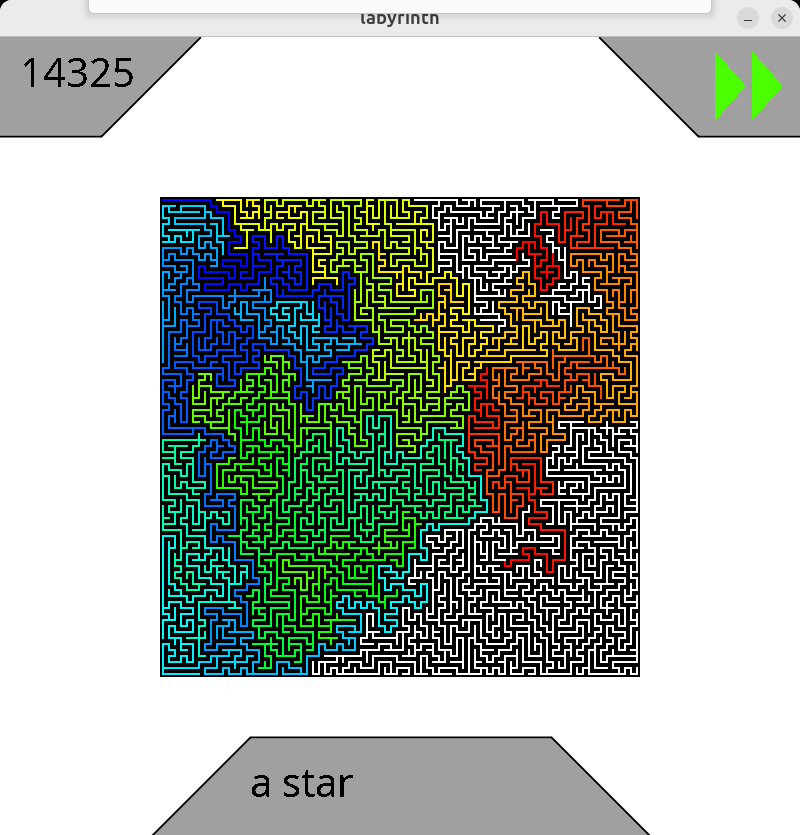
\includegraphics[width=0.8\textwidth]{java2d.png}}
    \caption{Przykładowa graficzna reprezentacja labiryntu wraz z szukaniem przez algorytm ścieżek wyjścia dla algorytmu A* w java2D. W lewym górnym rogu numer obecnie obecnie wykonywanego kroku.}
\end{figure}

Po zakończeniu działania programu można użyć następującej komendy, aby wygenerować wykresy porównujące algorytmy:

\begin{lstlisting}[caption=Generowanie wykresów]
python3 generate_plots.py
\end{lstlisting}

Komenda ta tworzy wykresy, które przedstawiają porównanie skuteczności algorytmów BFS, DFS, Dijkstra oraz A*. 

\begin{figure}[H]
    \centering
    \fbox{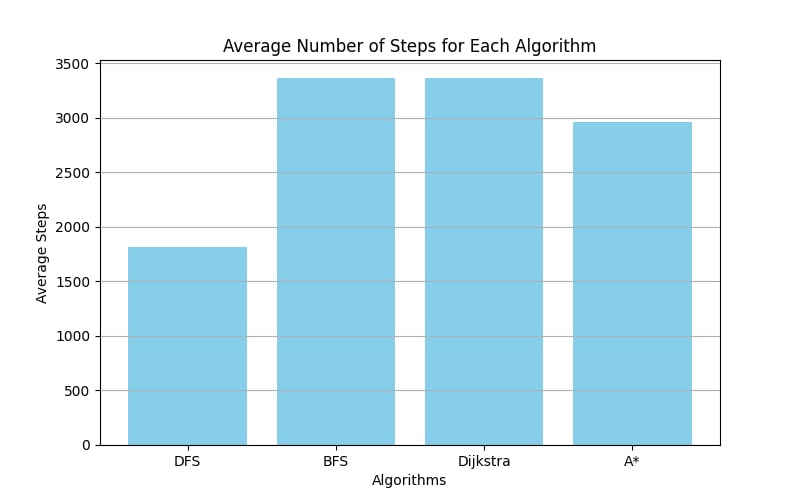
\includegraphics[width=0.8\textwidth]{avg_num_of_steps.png}}
    \caption{Średnia liczba kroków algorytmów BFS, DFS, Dijkstra i A*.}
\end{figure}

\begin{figure}[H]
    \centering
    \fbox{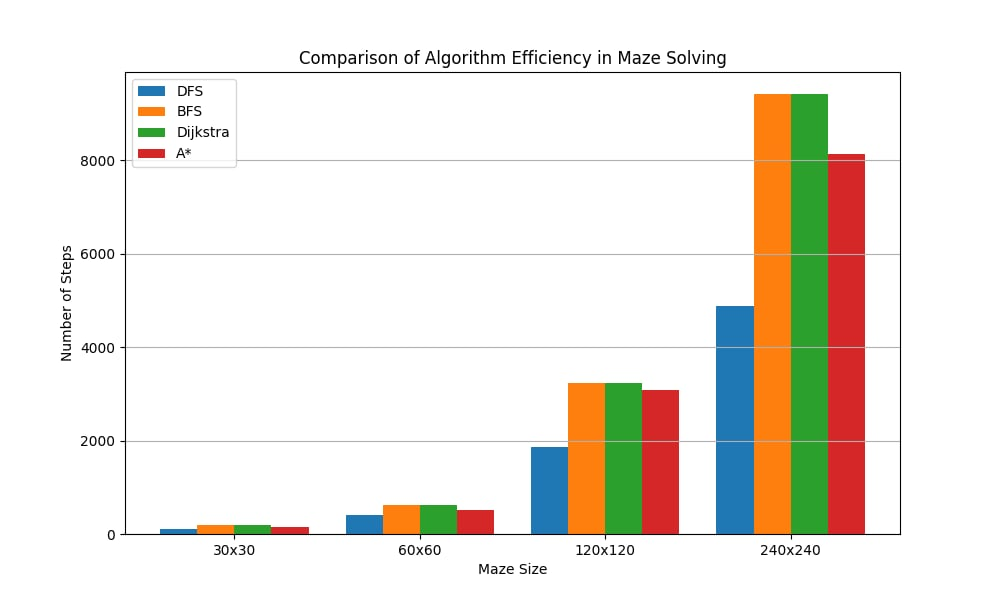
\includegraphics[width=0.8\textwidth]{comparison_efficiency.png}}
    \caption{Porównanie skuteczności algorytmów w rozwiązywaniu labiryntu na wykresach słupkowych.}
\end{figure}

\begin{figure}[H]
    \centering
    \fbox{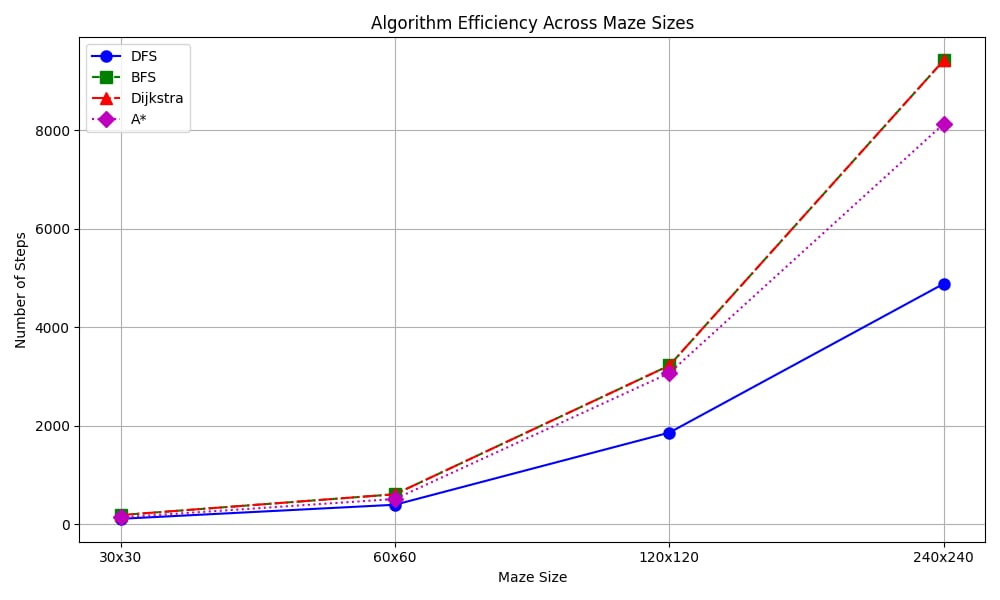
\includegraphics[width=0.8\textwidth]{efficiency_maze_sizes.png}}
    \caption{Porównanie skuteczności algorytmów w rozwiązywaniu labiryntu na wykresie liniowym.}
\end{figure}

\end{document}
